%Version 3.1 December 2024
% See section 11 of the User Manual for version history
%
%%%%%%%%%%%%%%%%%%%%%%%%%%%%%%%%%%%%%%%%%%%%%%%%%%%%%%%%%%%%%%%%%%%%%%
%%                                                                 %%
%% Please do not use \input{...} to include other tex files.       %%
%% Submit your LaTeX manuscript as one .tex document.              %%
%%                                                                 %%
%% All additional figures and files should be attached             %%
%% separately and not embedded in the \TeX\ document itself.       %%
%%                                                                 %%
%%%%%%%%%%%%%%%%%%%%%%%%%%%%%%%%%%%%%%%%%%%%%%%%%%%%%%%%%%%%%%%%%%%%%

%%\documentclass[referee,sn-basic]{sn-jnl}% referee option is meant for double line spacing

%%=======================================================%%
%% to print line numbers in the margin use lineno option %%
%%=======================================================%%

%%\documentclass[lineno,pdflatex,sn-basic]{sn-jnl}% Basic Springer Nature Reference Style/Chemistry Reference Style

%%=========================================================================================%%
%% the documentclass is set to pdflatex as default. You can delete it if not appropriate.  %%
%%=========================================================================================%%

%%\documentclass[sn-basic]{sn-jnl}% Basic Springer Nature Reference Style/Chemistry Reference Style

%%Note: the following reference styles support Namedate and Numbered referencing. By default the style follows the most common style. To switch between the options you can add or remove �Numbered� in the optional parenthesis. 
%%The option is available for: sn-basic.bst, sn-chicago.bst%  
 
%%\documentclass[pdflatex,sn-nature]{sn-jnl}% Style for submissions to Nature Portfolio journals
\documentclass[pdflatex,sn-basic]{sn-jnl}% Basic Springer Nature Reference Style/Chemistry Reference Style
%%\documentclass[pdflatex,sn-mathphys-num]{sn-jnl}% Math and Physical Sciences Numbered Reference Style
%%\documentclass[pdflatex,sn-mathphys-ay]{sn-jnl}% Math and Physical Sciences Author Year Reference Style
%%\documentclass[pdflatex,sn-aps]{sn-jnl}% American Physical Society (APS) Reference Style
%%\documentclass[pdflatex,sn-vancouver-num]{sn-jnl}% Vancouver Numbered Reference Style
%%\documentclass[pdflatex,sn-vancouver-ay]{sn-jnl}% Vancouver Author Year Reference Style
%%\documentclass[pdflatex,sn-apa]{sn-jnl}% APA Reference Style
%%\documentclass[pdflatex,sn-chicago]{sn-jnl}% Chicago-based Humanities Reference Style

%%%% Standard Packages
%%<additional latex packages if required can be included here>

\usepackage{graphicx}%
\usepackage{multirow}%
\usepackage{amsmath,amssymb,amsfonts}%
\usepackage{amsthm}%
\usepackage{mathrsfs}%
\usepackage[title]{appendix}%
\usepackage{xcolor}%
\usepackage{textcomp}%
\usepackage{manyfoot}%
\usepackage{booktabs}%
\usepackage{algorithm}%
\usepackage{algorithmicx}%
\usepackage{algpseudocode}%
\usepackage{listings}%
%%%%
\usepackage{tabularx}
\usepackage{booktabs}
\usepackage[justification=raggedright,singlelinecheck=false]{caption}
\usepackage{float}
\usepackage{enumitem}
%%%%%=============================================================================%%%%
%%%%  Remarks: This template is provided to aid authors with the preparation
%%%%  of original research articles intended for submission to journals published 
%%%%  by Springer Nature. The guidance has been prepared in partnership with 
%%%%  production teams to conform to Springer Nature technical requirements. 
%%%%  Editorial and presentation requirements differ among journal portfolios and 
%%%%  research disciplines. You may find sections in this template are irrelevant 
%%%%  to your work and are empowered to omit any such section if allowed by the 
%%%%  journal you intend to submit to. The submission guidelines and policies 
%%%%  of the journal take precedence. A detailed User Manual is available in the 
%%%%  template package for technical guidance.
%%%%%=============================================================================%%%%

%% as per the requirement new theorem styles can be included as shown below
\theoremstyle{thmstyleone}%
\newtheorem{theorem}{Theorem}%  meant for continuous numbers
%%\newtheorem{theorem}{Theorem}[section]% meant for sectionwise numbers
%% optional argument [theorem] produces theorem numbering sequence instead of independent numbers for Proposition
\newtheorem{proposition}[theorem]{Proposition}% 
%%\newtheorem{proposition}{Proposition}% to get separate numbers for theorem and proposition etc.

\theoremstyle{thmstyletwo}%
\newtheorem{example}{Example}%
\newtheorem{remark}{Remark}%

\theoremstyle{thmstylethree}%
\newtheorem{definition}{Definition}%

\raggedbottom
%%\unnumbered% uncomment this for unnumbered level heads

\begin{document}

\title[Article Title]{Real Options Approach to Valuation and Decision-making of E\&P Projects Under Geological and Market Uncertainties}

%%=============================================================%%
%% GivenName	-> \fnm{Joergen W.}
%% Particle	-> \spfx{van der} -> surname prefix
%% FamilyName	-> \sur{Ploeg}
%% Suffix	-> \sfx{IV}
%% \author*[1,2]{\fnm{Joergen W.} \spfx{van der} \sur{Ploeg} 
%%  \sfx{IV}}\email{iauthor@gmail.com}
%%=============================================================%%

\author*[1,3]{\fnm{Wellington} \sur{Nascimento}}\email{wellington@aluno.puc-rio.br}

\author[2]{\fnm{Reidar} \sur{Bratvold}}\email{reidar.bratvold@uis.no}
%%\equalcont{These authors contributed equally to this work.}

\author[1]{\fnm{Marco} \sur{Dias}}\email{marcoagd@ele.puc-rio.br}
%%\equalcont{These authors contributed equally to this work.}

\author[1]{\fnm{Marco} \sur{Pacheco}}\email{marco@ele.puc-rio.br}
%\equalcont{These authors contributed equally to this work.}

\affil[1]{\orgdiv{Department of Electrical Engineering}, \orgname{PUC-Rio}, \orgaddress{\street{Rua Marquês de São Vicente, 225}, \city{Rio de Janeiro}, \postcode{22451-900}, \state{RJ}, \country{Brazil}}}

\affil[2]{\orgdiv{Department of Energy Resources}, \orgname{University of Stavanger}, \orgaddress{\street{Rennebergstien 30}, \city{Stavanger}, \postcode{4021}, \state{Rogaland}, \country{Norway}}}

\affil[3]{\orgdiv{Petrobras}, \orgname{E\&P}, \orgaddress{\street{Av. Henrique Valadares, 28}, \city{Rio de Janeiro}, \postcode{20231-030}, \state{RJ}, \country{Brazil}}}

%%==================================%%
%% Sample for unstructured abstract %%
%%==================================%%

\abstract{The abstract serves both as a general introduction to the topic and as a brief, non-technical summary of the main results and their implications. Authors are advised to check the author instructions for the journal they are submitting to for word limits and if structural elements like subheadings, citations, or equations are permitted.}

%%================================%%
%% Sample for structured abstract %%
%%================================%%

 %\abstract{\textbf{Purpose:} The abstract serves both as a general introduction to the topic and as a brief, non-technical summary of the main results and their implications. The abstract must not include subheadings (unless expressly permitted in the journal's Instructions to Authors), equations or citations. As a guide the abstract should not exceed 200 words. Most journals do not set a hard limit however authors are advised to check the author instructions for the journal they are submitting to.
% 
% \textbf{Methods:} The abstract serves both as a general introduction to the topic and as a brief, non-technical summary of the main results and their implications. The abstract must not include subheadings (unless expressly permitted in the journal's Instructions to Authors), equations or citations. As a guide the abstract should not exceed 200 words. Most journals do not set a hard limit however authors are advised to check the author instructions for the journal they are submitting to.
% 
% \textbf{Results:} The abstract serves both as a general introduction to the topic and as a brief, non-technical summary of the main results and their implications. The abstract must not include subheadings (unless expressly permitted in the journal's Instructions to Authors), equations or citations. As a guide the abstract should not exceed 200 words. Most journals do not set a hard limit however authors are advised to check the author instructions for the journal they are submitting to.
% 
% \textbf{Conclusion:} The abstract serves both as a general introduction to the topic and as a brief, non-technical summary of the main results and their implications. The abstract must not include subheadings (unless expressly permitted in the journal's Instructions to Authors), equations or citations. As a guide the abstract should not exceed 200 words. Most journals do not set a hard limit however authors are advised to check the author instructions for the journal they are submitting to.}

\keywords{keyword1, Keyword2, Keyword3, Keyword4}

%%\pacs[JEL Classification]{D8, H51}

%%\pacs[MSC Classification]{35A01, 65L10, 65L12, 65L20, 65L70}

\maketitle

\section{Introduction}\label{sec1}

The Introduction section, of referenced text \cite{bib1} expands on the background of the work (some overlap with the Abstract is acceptable). The introduction should not include subheadings.

Springer Nature does not impose a strict layout as standard however authors are advised to check the individual requirements for the journal they are planning to submit to as there may be journal-level preferences. When preparing your text please also be aware that some stylistic choices are not supported in full text XML (publication version), including coloured font. These will not be replicated in the typeset article if it is accepted. 

The remainder of the paper is organized as follows. A literature review is presented in Section \ref{sec2}, followed by a detailed description of the problem in Section \ref{sec23}. Section \ref{sec4} outlines the methodology, which includes the assumption of the Geometric Brownian Motion (GBM) for variable operating costs, Two-Factor model for oil prices, a geological benchmark model (Egg model), Monte Carlo Simulation (MCS) and Least Squares Monte Carlo (LSM) to estimate the project's value with options. The results and related discussions are presented in Section \ref{sec5}. Finally, Section \ref{sec6} concludes the paper with suggestions for potential future research.

\section{Literature Review}\label{sec2}

Theory of investment under uncertainty, as developed by \cite{ref1}, provides the real options approach (ROA) for evaluating irreversible investment decisions in uncertain environments. In the context of petroleum exploration and production (E\&P) industry, this approach emphasizes the value of managerial flexibility in timing investments, accounting for volatility in prices, geological information, and regulatory factors. Unlike traditional Discounted Cash Flow (DCF) method, the ROA captures the strategic value of waiting and learning before committing capital.

\cite{ref2} advances the ROA by integrating financial option pricing with strategic investment analysis, providing a comprehensive approach for valuing flexibility in corporate decision-making. In relation to E\&P projects, \cite{ref2} highlights how embedded options, such as the option to defer, expand, or abandon projects, can significantly alter investment valuation under uncertainty, particularly in capital-intensive and high-risk environments like oil and gas industry.

\cite{ref3} presents a comprehensive overview of ROA for valuing E\&P assets under market and technical uncertainty. Through intuitive examples and practical applications, the paper emphasizes the value of managerial flexibility, discussing key decisions such as drilling, appraisal, and production expansion. It also reviews classical and advanced stochastic models for oil price behavior and their implications for optimal investment strategies. \cite{ref4} present a detailed case study of an offshore E\&P project, incorporating sequential exploration, appraisal, scaling, and abandonment options under joint geological and market uncertainty. Their findings show that traditional DCF methods underestimate project value by ignoring embedded flexibilities, particularly the option to abandon, which proved to be the most valuable under mean-reverting oil price scenarios. Complementing this, \cite{ref5} integrates government incentives—such as royalty relief and price/volume-based royalty schemes—into a ROA, demonstrating that these mechanisms not only enhance the economic viability of high-risk prospects but also reduce the project's critical investment thresholds. 

There are several numerical approaches to support early-stage decision-making in oil field development under uncertainty. \cite{ref6} propose an numerical optimization-based approach incorporating Latin Hypercube Sampling and stochastic oil price model to evaluate how geological and economic uncertainties influence key field design variables. Their results show that while early-stage designs may be conservative and suboptimal, they offer lower financial risk, and the value of perfect information is often limited. \cite{ref7} develop a compound ROA to assess tieback investments for marginal oil and gas fields on the Norwegian Continental Shelf, accounting for reservoir and price uncertainty. By modeling a portfolio of sequential investment decisions and incorporating updates in reservoir size and oil prices, their approach demonstrates that flexible strategies can significantly outperform static valuations, increasing returns by over 25\%. These contributions emphasize the value of integrating uncertainty modeling, managerial flexibility with ROA to enhance capital allocation in upstream projects.

\cite{ref8} accentuate for a paradigm shift in petroleum investment evaluation, emphasizing the value of flexibility under uncertainty through ROA. They examine the dominance of traditional NPV methods and presents a structured comparison of ROA, including the Marketed Asset Disclaimer (MAD) and integrated frameworks. It highlights how managerial flexibilities—such as timing, expansion, and abandonment—can be systematically valued, offering strategic insight and higher project value when properly exercised. \cite{ref9} argue that conventional valuation techniques, such as DCF and Value of Information (VoI), often fail to capture the full economic potential of oil and gas investments under uncertainty. They introduce the concept of Value of Flexibility (VoF) as a complement to VoI, pointing out the strategic value of embedding flexibility in project design to manage or exploit uncertainty. Using practical examples, the authors demonstrate how flexibility in development timing, capacity scaling, and operational decisions can significantly increase project value, advocating for a shift from valuation to value creation through real options thinking. \cite{ref10} analyze the disconnect between improvements in uncertainty quantification and the lack of corresponding advances in decision quality within the oil and gas industry. Based on a survey of 494 professionals, they find that while probabilistic modeling has increased, it has not translated into better decisions, largely due to the misconception that more detailed modeling inherently improves outcomes. The authors propose a decision-focused approach emphasizing clarity, flexibility, and value-driven analysis over excessive modeling detail. They advise for iterative, decision-oriented processes and broader adoption of VoI and decision analysis techniques to truly improve decision-making effectiveness. \cite{ref11} propose a novel approach for managing risk in petroleum development by integrating ROA with dynamic programming through the Bellman equation. This mathematical union enables optimal policy development along branching, sequential investment pathways typical of oil and gas projects. Applied to a Central Asian gas condensate field, the approach demonstrates how investment flexibility, particularly in production expansion, can be systematically evaluated to support more robust decision-making under uncertainty.

\cite{ref12} propose a decision-analytic approach for valuing real options using binomial decision trees instead of traditional binomial lattices. This approach allows for intuitive modeling of managerial flexibility by integrating risk-neutral valuation with decision tree structures, making it suitable for problems involving multiple uncertainties and complex options. Applied to an oil production case, the method demonstrates how simulation-based volatility estimation and dynamic programming can produce flexible, transparent, and computationally practical ROA. \cite{ref13} critiques the binomial decision tree method proposed by \cite{ref12} for solving real-options problems, identifying both practical and conceptual limitations. He argues for more consistent use of fully risk-neutral valuation, and recommends binomial lattices over decision trees for computational efficiency and clarity. He also highlight that estimating volatility via discounted cash flow simulations may overstate option values, and promote advanced methods, such as LSM proposed by \cite{ref14} to more accurately capture project uncertainty and optimize real investment decisions.

In this paper, we aim to generalize the problem addressed by \cite{ref12}, hereafter referred to as BDH problem, incorporating the methodological proposed by \cite{ref13} and with the addition of more flexibility to the problem. While the original analysis focuses on exercising flexibility at a particular year, namely Year 5, we extend the ROA to allow for managerial flexibility throughout the entire production period of the oil project. By doing so, we demonstrate that greater flexibility leads to higher project value, consistent with findings in the \cite{ref9}. Additionally, uncertainties will be incorporated into the geological model, thereby introducing variability in the production curve, thus aligning the problem more closely with real projects scenarios. The next section provides a detailed description of the problem setup.

\section{Problem Description}\label{sec23}

BDH problem, addressed in \cite{ref12}, involves the evaluation of an oil production project using ROA. They illustrate the application of a binomial decision tree approach to this problem. The project comprises an estimated reserve of 90 million barrels, with an initial production of 9 million barrels per year that declines at a rate of 15\% annually over a 10-year horizon. Variable operating costs start at \$10 per barrel and increase by 2\% per year, while oil prices begin at \$25 per barrel and grow at 3\% annually. A fixed annual cost of \$5 million is also included. The analysis uses a 10\% risk-adjusted discount rate and a 5\% risk-free rate. These data and the resulting base case cash flows are summarized in Table \ref{tab1}.


\begin{table}[h]
\centering
\caption{Base Case Expected Cash Flows for the Project}\label{tab1}%
\begin{tabularx}{13.5cm}{l *{11}{>{\centering\arraybackslash}X}}
\toprule
\textbf{Year} & \textbf{0} & \textbf{1} & \textbf{2} & \textbf{3} & \textbf{4} & \textbf{5} & \textbf{6} & \textbf{7} & \textbf{8} & \textbf{9} & \textbf{10} \\
\midrule
Remaining Reserves              &  90.0   & 90.0 & 81.0 & 73.4 & 66.8 & 61.3 & 56.6 & 52.6 & 49.2 & 46.3 & 43.9 \\
Production Level              &     & 9.0 & 7.7 & 6.5 & 5.5 & 4.7 & 4.0 & 3.4 & 2.9 & 2.5 & 2.1 \\
Variable Op Cost Rate         &  10.0  & 10.2 & 10.4 & 10.6 & 10.8 & 11.0 & 11.3 & 11.5 & 11.7 & 12.0 & 12.2 \\
Oil Price                     & 25.0  & 25.8 & 26.5 & 27.3 & 28.1 & 29.0 & 29.9 & 30.7 & 31.7 & 32.6 & 33.6 \\
\addlinespace
Revenues                      &     & 231.8 & 202.9 & 177.6 & 155.5 & 136.2 & 119.2 & 104.4 & 91.4 & 80.0 & 70.0 \\
Production Cost               &     & (96.8) & (84.6) & (74.0) & (64.8) & (56.9) & (50.0) & (44.0) & (38.8) & (34.3) & (30.4) \\
\cmidrule{3-12}
Cash Flow                     &     & 135.0 & 118.3 & 103.6 & 90.7 & 79.3 & 69.2 & 60.4 & 52.6 & 45.7 & 39.6 \\
Profit Sharing                &     & (33.7) & (29.6) & (25.9) & (22.7) & (19.8) & (17.3) & (15.1) & (13.1) & (11.4) & (9.9) \\
\cmidrule{3-12}
\addlinespace
\textbf{Net Cash Flows}       &  & \textbf{101.2} & \textbf{88.7} & \textbf{77.7} & \textbf{68.0} & \textbf{59.5} & \textbf{51.9} & \textbf{45.3} & \textbf{39.4} & \textbf{34.3} & \textbf{29.7} \\
\addlinespace
PV of Cash Flows              & \textbf{404.0} & 444.5 & 377.6 & 317.7 & 264.0 & 215.6 & 171.7 & 131.8 & 95.1 & 61.3 & 29.7 \\
Cash Flow Ratios          &    & 0.228 & 0.235 & 0.245 & 0.258 & 0.276 & 0.302 & 0.344 & 0.414 & 0.559 & 1.000  \\
\bottomrule
\end{tabularx}
\footnotetext{Source: Adapted from \cite{ref12}.}
\end{table}

Expected cash flows are first calculated using DCF methods, resulting in a base-case project value of \$404 million. MCS is then performed, incorporating uncertainties in oil prices and operating costs, both modeled as GBM. This yields an estimated project return volatility of 46.6\%, which is used to build the binomial decision tree.

Decision tree framework enables the modeling of managerial flexibility through ROA. For example, the firm may divest the project in Year 5 for \$100 million or buy out a partner's 25\% share for \$40 million. These options increase the project value to \$444.9 million. The model also allows for the incorporation of private risks, such as uncertainty related to water breakthrough in the reservoir, and the impact of managerial risk aversion through the use of utility functions \citep{ref12}. This example demonstrates the practical applicability and flexibility of the BDH problem in capturing both market and private risks, as well as the value of strategic decision-making under uncertainty.

BDH problem is revisited in \cite{ref13} under a fully risk-neutral valuation approach. In this version of the problem, oil prices are treated as market risks and are assumed to follow a risk-neutral growth rate of 0\% per year. Variable operating costs, on the other hand, are assumed to be private risks, uncorrelated with market variables, and follow their actual process. Assuming the decision maker is risk neutral, the integrated valuation procedure combines the risk-neutral process for market risks with the true process for private risks. This setup results in the same valuation as that produced by the equilibrium approach, meaning both lead to an identical fully risk-neutral valuation model. The input parameters and resulting cash flows for this formulation are detailed in Table \ref{tab2}.

\begin{table}[h]
\centering
\caption{A Risk-Neutral Version of BDH's Base Case Analysis}\label{tab2}%
\begin{tabularx}{13.5cm}{l *{11}{>{\centering\arraybackslash}X}}
\toprule
\textbf{Year} & \textbf{0} & \textbf{1} & \textbf{2} & \textbf{3} & \textbf{4} & \textbf{5} & \textbf{6} & \textbf{7} & \textbf{8} & \textbf{9} & \textbf{10} \\
\midrule
Production Level              &     & 9.0 & 7.7 & 6.5 & 5.5 & 4.7 & 4.0 & 3.4 & 2.9 & 2.5 & 2.1 \\
Variable Op Cost Rate         &  10.0   & 10.2 & 10.4 & 10.6 & 10.8 & 11.0 & 11.3 & 11.5 & 11.7 & 12.0 & 12.2 \\
Oil Price                     & 25.0  & 25.0 & 25.0 & 25.0 & 25.0 & 25.0 & 25.0 & 25.0 & 25.0 & 25.0 & 25.0 \\
\addlinespace
Revenues                      &     & 225.0 & 191.3 & 162.6 & 138.2 & 117.5 & 99.8 & 84.9 & 72.1 & 61.3 & 52.1 \\
Production Cost               &     & (96.8) & (84.6) & (74.0) & (64.8) & (56.9) & (50.0) & (44.0) & (38.8) & (34.3) & (30.4) \\
\cmidrule{3-12}
Cash Flow                     &     & 128.2 & 106.7 & 88.6 & 73.4 & 60.6 & 49.9 & 40.9 & 33.3 & 27.0 & 21.7 \\
Profit Sharing                &     & (32.1) & (26.7) & (22.1) & (18.3) & (15.1) & (12.5) & (10.2) & (8.3) & (6.8) & (5.4) \\
\cmidrule{3-12}
\addlinespace
\textbf{Net Cash Flows}       &  & \textbf{96.2} & \textbf{80.0} & \textbf{66.4} & \textbf{55.0} & \textbf{45.4} & \textbf{37.4} & \textbf{30.7} & \textbf{25.0} & \textbf{20.3} & \textbf{16.3} \\
\addlinespace
PV of Cash Flows              & \textbf{392.0} & 411.6 & 331.2 & 263.8 & 207.3 & 159.9 & 120.6 & 86.9 & 59.0 & 35.8 & 16.3 \\
Cash Flow Ratios          &    & 0.233 & 0.241 & 0.251 & 0.265 & 0.284 & 0.311 & 0.352 & 0.423 & 0.566 & 1.000  \\
\bottomrule
\end{tabularx}
\footnotetext{Source: Adapted from \cite{ref13}.}
\end{table}

Using this approach, the value of the investment is simply the expected NPV, calculated using the risk-neutral valuation and discounted at the risk-free rate of 5\% per year. For projects without options, a deterministic model, such as one based on expected values of oil prices and costs, can be used to compute NPV. In this case, the oil production example leads to an NPV of \$392 million under the risk-neutral approach, as compared to \$404 million from the risk-adjusted DCF analysis of \cite{ref12}.

The discrepancy between the two NPV stems from fundamental differences in how future revenues and costs are valued. In the traditional DCF approach used by \cite{ref12}, oil prices are assumed to grow at 3\% annually and are discounted at a 10\% risk-adjusted rate, resulting in a net annual decline in the present value of future revenues by 7\%. In contrast, the risk-neutral approach assumes no growth in oil prices and applies a lower, risk-free discount rate of 5\%, leading to a slower decline in present value—only 5\% per year. This implies that the risk-neutral method assigns relatively greater weight to future oil revenues. However, because future operating costs are not risk-adjusted and are also discounted at the lower risk-free rate, their present value increases under the risk-neutral approach. In this specific example, the effect of higher-valued future costs outweighs the benefit of more highly valued revenues, leading to a lower overall NPV. Nevertheless, in other situations, such as E\&P projects where most of the production occurs farther into the future, the increased emphasis on long-term revenues could dominate, potentially resulting in a higher valuation using the risk-neutral approach.

\cite{ref13} discusses how to determine an optimal exercise policy for ROA by evaluating the expected continuation value of each available alternative at each decision point, conditioned on the information available at that time. The continuation value represents the expected NPV of future cash flows if a specific decision is made. The optimal policy is the one that selects the alternative with the highest continuation value given the current state. To implement this in practice, \cite{ref13} adopts the LSM approach proposed by \cite{ref14}, which estimates continuation values through regression analysis based on simulation results.

In the context BDH problem, this method involves simulating the project under the assumption that no options are exercised, for example, continuing operations without divesting or buying out a partner. At the decision point in Year 5, for each simulation run, the NPV of the remaining cash flows (i.e., the realized continuation value) is recorded along with the oil price and variable operating cost in that scenario. A regression is then performed with the continuation value as the dependent variable and the state variables (oil price and cost) as independent variables. Using the fully risk-neutral approach, \cite{ref13} conducts a simulation with 10,000 trials and obtains an estimated regression equation that expresses the continuation value as a function of the observed state variables at the time of the decision. This equation can then be used to support near-optimal decision-making by comparing the estimated continuation value with the value of exercising the option, choosing the alternative with the highest expected value.

In \cite{ref15}, the authors analyze the LSM method for ROA, emphasizing the importance of regression function selection and path inclusion strategies. They demonstrate that excluding out-of-the-money paths can undervalue options, while higher-order polynomial regressions show robustness in only in-the-money/out-of-the-money cases. Notably, \cite{ref13}, who applied LSM to the BDH problem, used all simulated paths and a polynomial regression function, reinforcing the method's reliability when capturing full flexibility. He highlights LSM's effectiveness in sequential decision-making under uncertainty.

Another interesting result was obtained by \cite{ref16}, who developed an approach to determine the optimal timing for gas cap blowdown by explicitly modeling key sources of uncertainty and applying ROA in combination with the LSM method. The approach incorporates uncertainties in oil and gas prices, modeled using a two-factor model prices \citep{ref17} calibrated via Kalman filtering, as well as uncertainties related to reserves, variable operating costs, and transition costs. This integration enables flexible and adaptive decision-making over time and produces strategy maps that identify the most value-maximizing actions under a wide range of market and reservoir conditions. 

Based on the previously described BDH problem, we propose a revised formulation that enhances generality and realism through improved treatment of key parameters:
\begin{itemize}
    \item \textbf{Production level}: uncertainty in the production profile will be incorporated by employing the Egg model (Figure \ref{fig1}), a synthetic reservoir model comprising one deterministic and 100 stochastic permeability realizations, totaling 101 equiprobable scenarios \citep{ref18} and thereby capturing geological uncertainties;
    \item \textbf{Variable operational cost}: this parameter will be modeled as a stochastic process following a GBM, similar to the approaches in \cite{ref19}, \cite{ref20} and \cite{ref21};
    \item \textbf{Oil price}: the oil price dynamics will be captured using the two-factor model proposed by \cite{ref17}.
\end{itemize}

\begin{figure}[H]
\centering
\begin{minipage}{0.95\textwidth}
  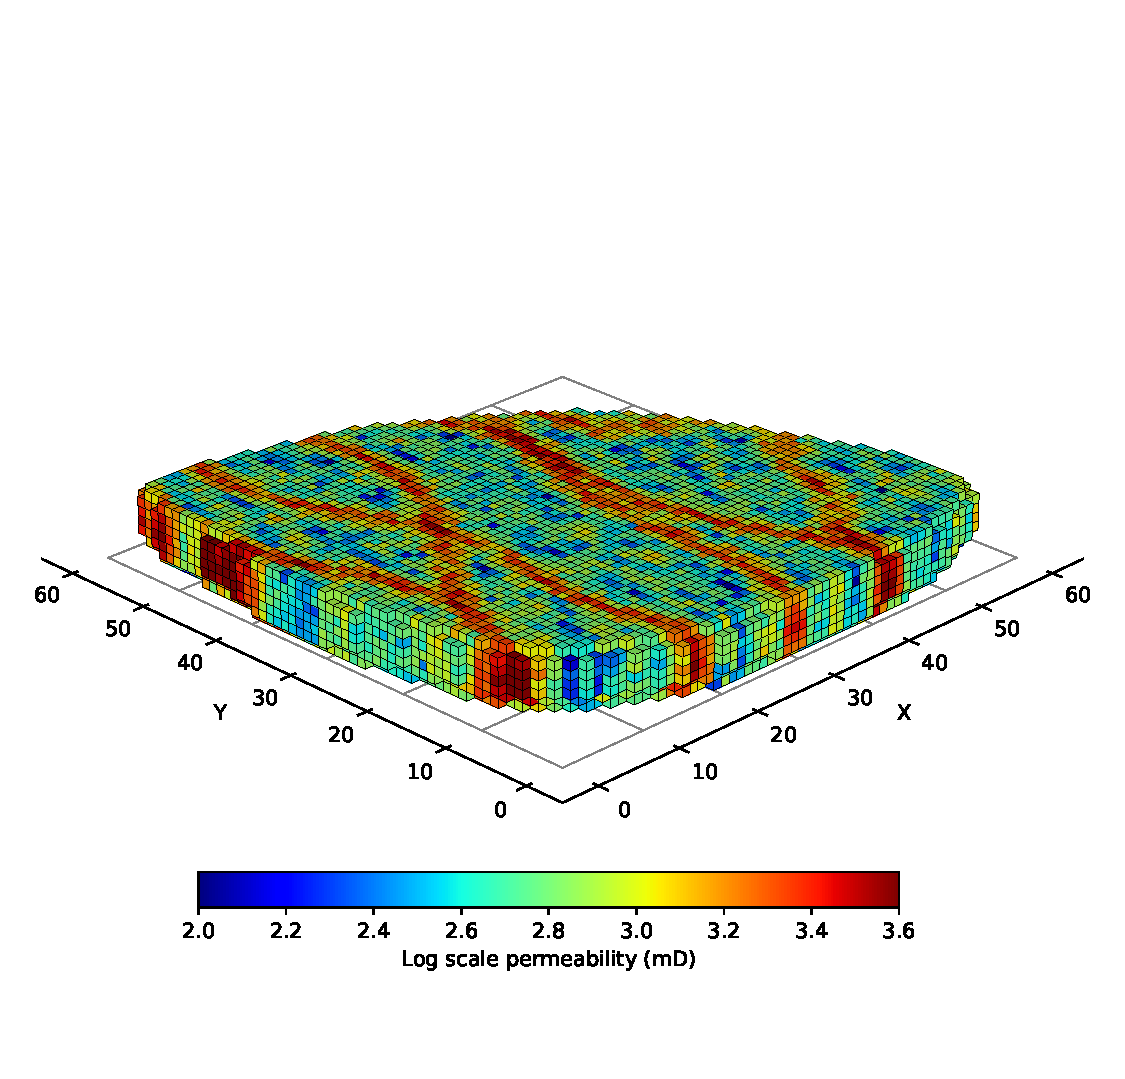
\includegraphics[width=\textwidth]{egg_model_log_3D.eps}
  \caption{The Egg model: permeability distribution of the deterministic version.}
  \label{fig1}
\end{minipage}
\end{figure}

The available decision options remain unchanged: \textit{buy out partner}, \textit{continue with current share}, or \textit{divest}. However, instead of restricting the exercise of these options to Year 5, we introduce greater flexibility by allowing them to be exercised at any time throughout the production period of the field.


\section{Methodology}\label{sec4}

Sample body text. Sample body text. Sample body text. Sample body text. Sample body text. Sample body text. Sample body text. Sample body text.

\begin{figure}[H]
\centering
\begin{minipage}{0.95\textwidth}
  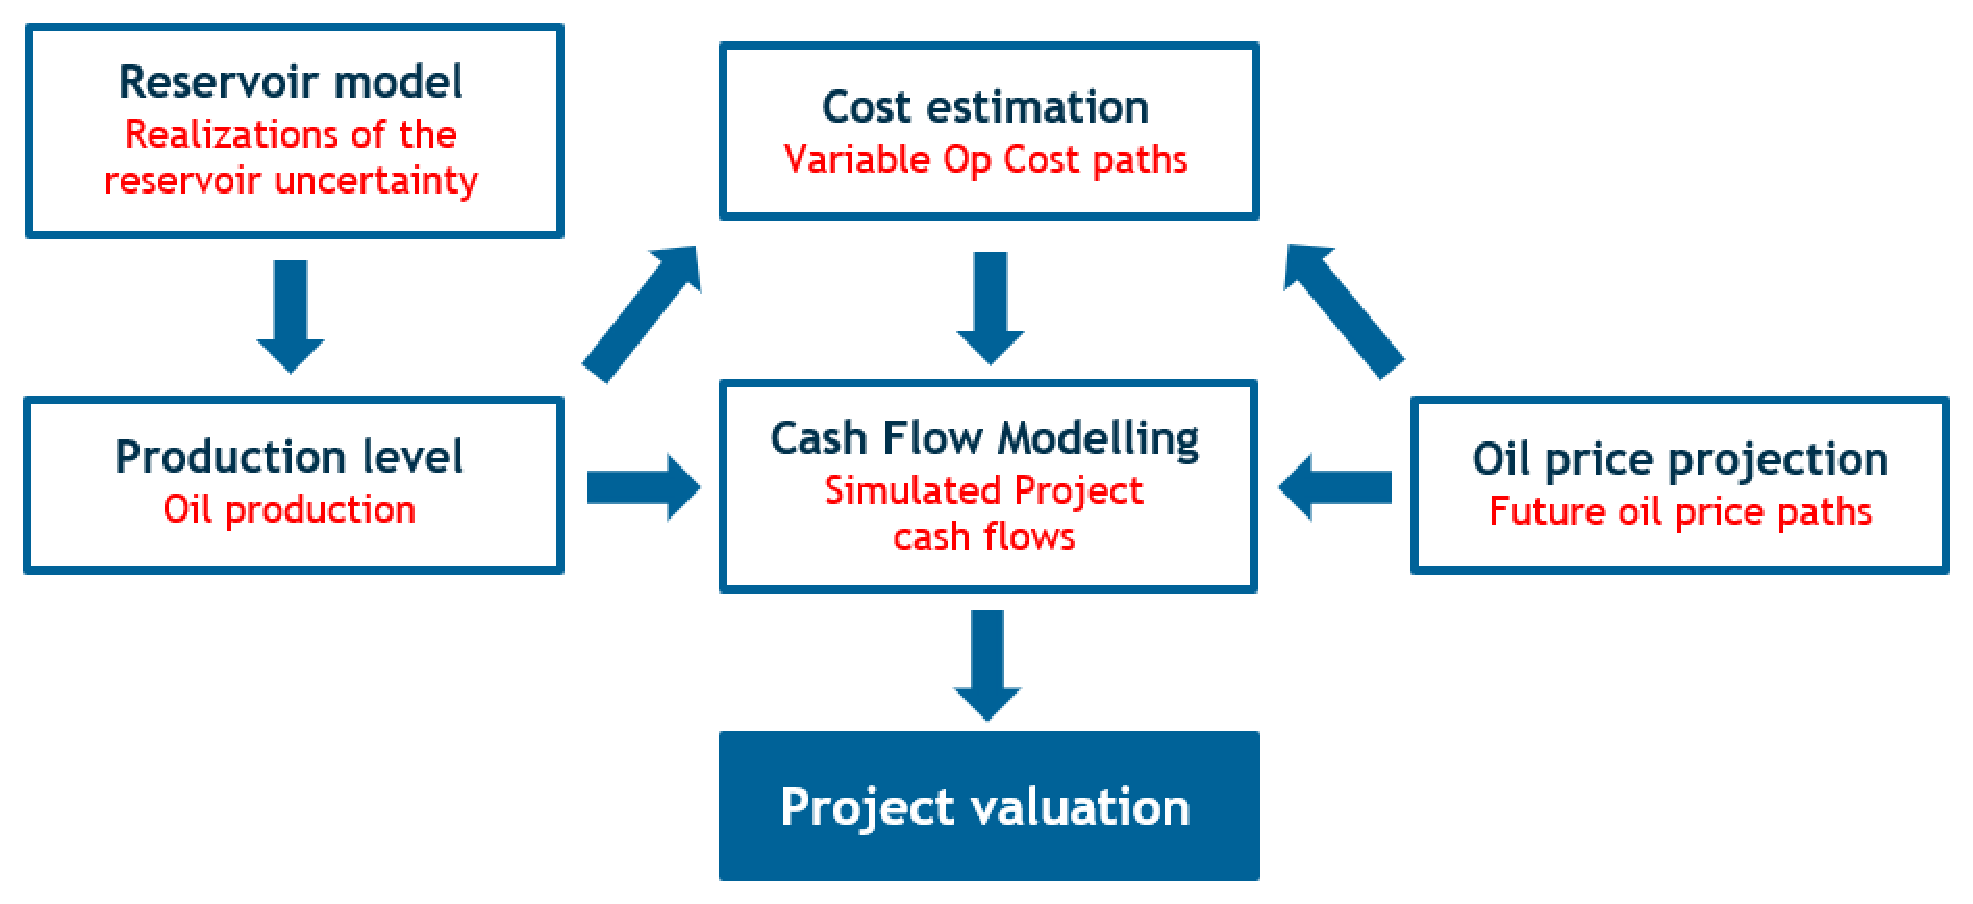
\includegraphics[width=\textwidth]{valuation.eps}
  \caption{The valuation procedure. Adapted from \cite{ref22}.}
  \label{fig2}
\end{minipage}
\end{figure}

\subsection{The Egg Model}\label{subsec41}

Egg Model, originally introduced by \cite{ref23} and further standardized by \cite{ref18}, is a widely used synthetic benchmark for reservoir simulation studies. The model comprises 25,200 gridblocks, of which 18,533 are active, forming an egg-shaped reservoir by excluding inactive gridblocks. Its reservoir architecture features a set of meandering, high-permeability channels embedded within a low-permeability matrix, thereby representing the geological complexity of fluvial depositional environments. Due to the high degree of vertical correlation among the seven layers, the permeability fields can be cosidered almost two dimensional. The standard configuration includes twelve wells, eight injectors and four producers (Figure \ref{fig3}), their locations being well documented in the literature.

\begin{figure}[H]
\centering
\begin{minipage}{0.95\textwidth}
  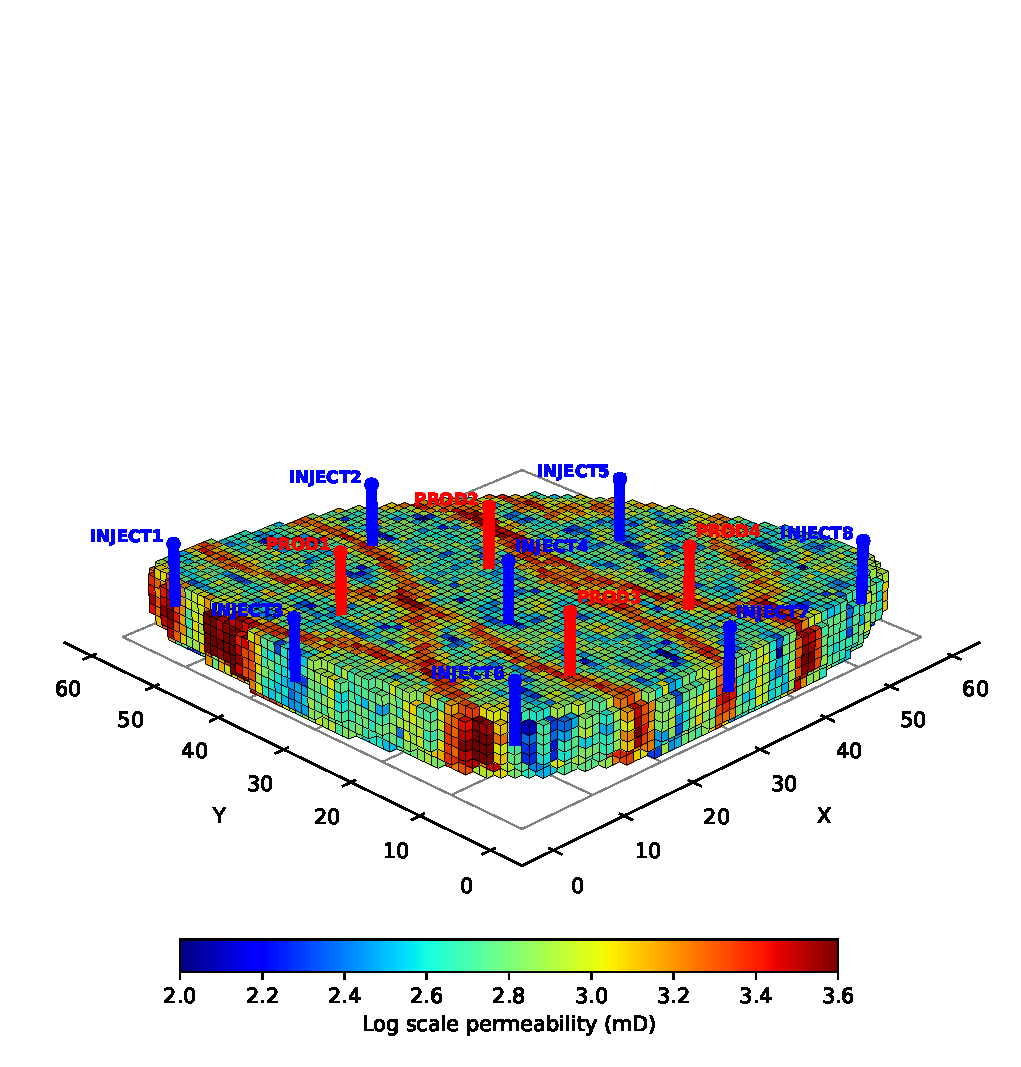
\includegraphics[width=\textwidth]{egg_model_log_3D_well.eps}
  \caption{Egg reservoir model. Blue lines are an indicator of injector wells, and red ones represent the producers.}
  \label{fig3}
\end{minipage}
\end{figure}

A distinctive feature of the Egg Model is the absence of both an aquifer and a gas cap, resulting in negligible primary production and making waterflooding the dominant recovery mechanism. The model has been constructed as an ensemble of 101 three-dimensional realizations, each with unique, hand-drawn permeability fields. This stochastic approach enables the evaluation of algorithms under geological uncertainty, providing a robust test bed for methods related to reservoir simulation, production optimization, history matching, and closed-loop reservoir management.

The dataset—including input files for various simulators and 100 additional permeability realizations—is publicly available to facilitate research and comparison of advanced reservoir management strategies. Details of the geological, fluid, and operational properties employed in this study are summarized in Table \ref{tab3}. Notably, the Corey model is adopted for calculating the oil and water relative permeabilities, with specific Corey exponents and endpoint values listed accordingly.

\begin{table}[h]
\centering
\caption{Reservoir and fluid properties for the Egg model.}
\label{tab3}
\begin{tabular}{lcl}
\hline
\textbf{Property} & \textbf{Value} & \textbf{Unit} \\
\hline
Dimensions & $60 \times 60 \times 7 = 25200$ & -- \\
Cell dimensions size & $8(x) \times 8(y) \times 4(z)$ & m \\
The maximum water injection rate & 79.5 & m$^3$/day \\
Production well bottom-hole pressure & $39.5 \times 10^6$ & Pa \\
Corey exponent for oil & 4 & -- \\
Corey exponent for water & 3 & -- \\
Connate water saturation & 20 & \% \\
Initial water saturation & 10 & \% \\
Residual oil saturation & 10 & \% \\
Endpoint relative permeability to oil & 0.8 & -- \\
Endpoint relative permeability to water & 0.75 & -- \\
Capillary pressure & 0 & Pa \\
Porosity & 0.2 & -- \\
Reservoir pressure & $40 \times 10^6$ & Pa \\
Oil compressibility & $1.0 \times 10^{-10}$ & Pa$^{-1}$ \\
Water compressibility & $1.0 \times 10^{-10}$ & Pa$^{-1}$ \\
Rock compressibility & 0 & Pa$^{-1}$ \\
Oil viscosity & $5.0 \times 10^{-3}$ & Pa$\cdot$s \\
Water viscosity & $5.0 \times 10^{-3}$ & Pa$\cdot$s \\
Simulation time & 3600 & day \\
\hline
\end{tabular}
\footnotetext{Source: Adapted from \cite{ref18}.}
\end{table}

Oil and water production profiles of the deterministic version (reference model) over a simulation period of 3600 days (10 years) are illustrated in Figure \ref{fig4}. During the initial production phase, no water production is observed, since the initial water saturation is set to 0.1, which is equal to the irreducible (connate) water saturation. After the onset of water production, the oil production rate exhibits a sharp decline, indicating the occurrence of water breakthrough. The breakthrough time varies among the production wells, highlighting the reservoir's heterogeneity. Therefore, the reliable prediction of water breakthrough times for each production well is essential for effective reservoir management and production optimization.

\begin{figure}[H]
\centering
\begin{minipage}{0.95\textwidth}
  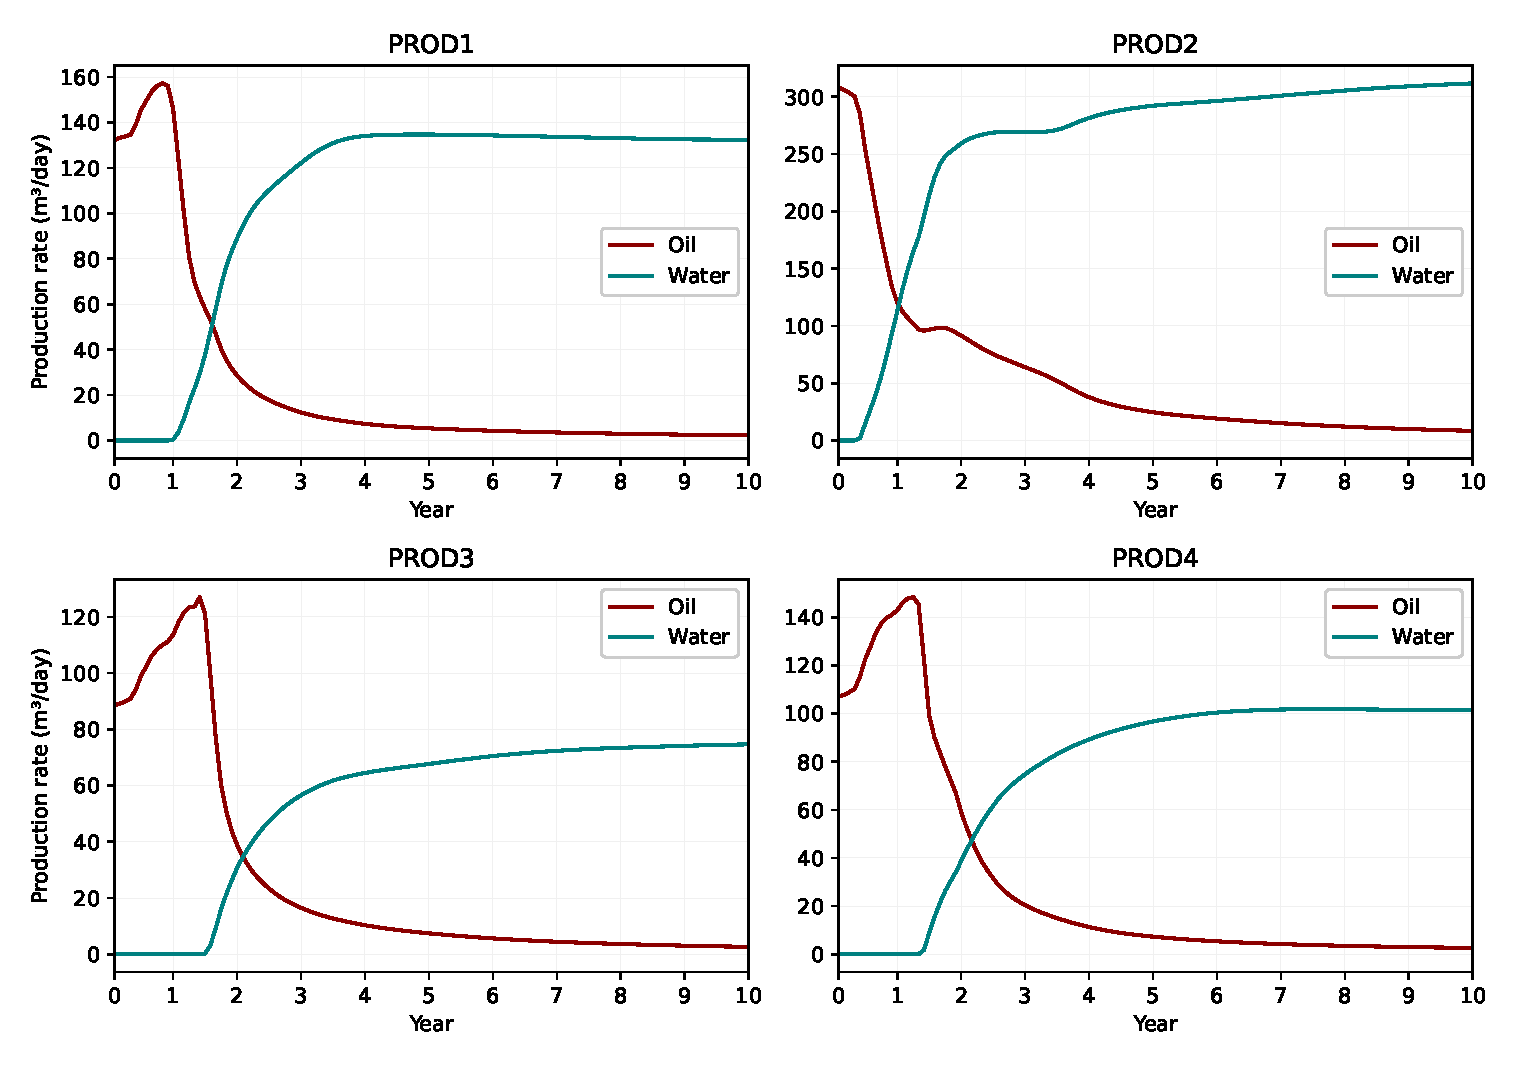
\includegraphics[width=\textwidth]{production_plot.eps}
  \caption{Oil and water production rates of the reference model for the four production wells.}
  \label{fig4}
\end{minipage}
\end{figure}

In this study, it is assumed that the vertical oil production well is fully penetrating. Accordingly, since there are 3,600 gridblocks in the first layer, of which 2,491 are active cells, this assumption yields 2,491 feasible well placement scenarios, corresponding to the number of active gridblocks in the top layer of the reservoir model. Figure \ref{fig5} illustrates the spatial distribuition of permeability in the top layer for 16 realizations of the Egg model. These realizations were randomly selected from the original set of 101, which consists of one reference field and one hundred initial stochastic models. The models exhibit high-permeability channels within a low-permeability background, with each realization presenting a distinct channel pattern.

\begin{figure}[H]
\centering
\begin{minipage}{0.95\textwidth}
  \includegraphics[width=\textwidth]{egg_model_log_2D_grid.eps}
  \caption{Permeability distribution maps for top layers of 25 realizations of the Egg model.}
  \label{fig5}
\end{minipage}
\end{figure}

\subsection{Monte Carlo Simulation}\label{subsec42}

Monte Carlo Simulation is a robust and flexible approach for uncertainty analysis, widely applied in decision-making within petroleum engineering (Bratvold et al.). The central idea of MCS is to propagate uncertainty from input parameters, such as costs, prices, and geological properties, to key output metrics like NPV, reserves, or production forecasts. By constructing probabilistic models for uncertain inputs and performing repeated sampling, MCS enables the generation of output distributions that provide valuable insights for risk-informed decisions. The general workflow of MCS, including input sampling and output analysis, is illustrated in Figure \ref{fig6}.

\begin{figure}[H]
\centering
\begin{minipage}{0.85\textwidth}
  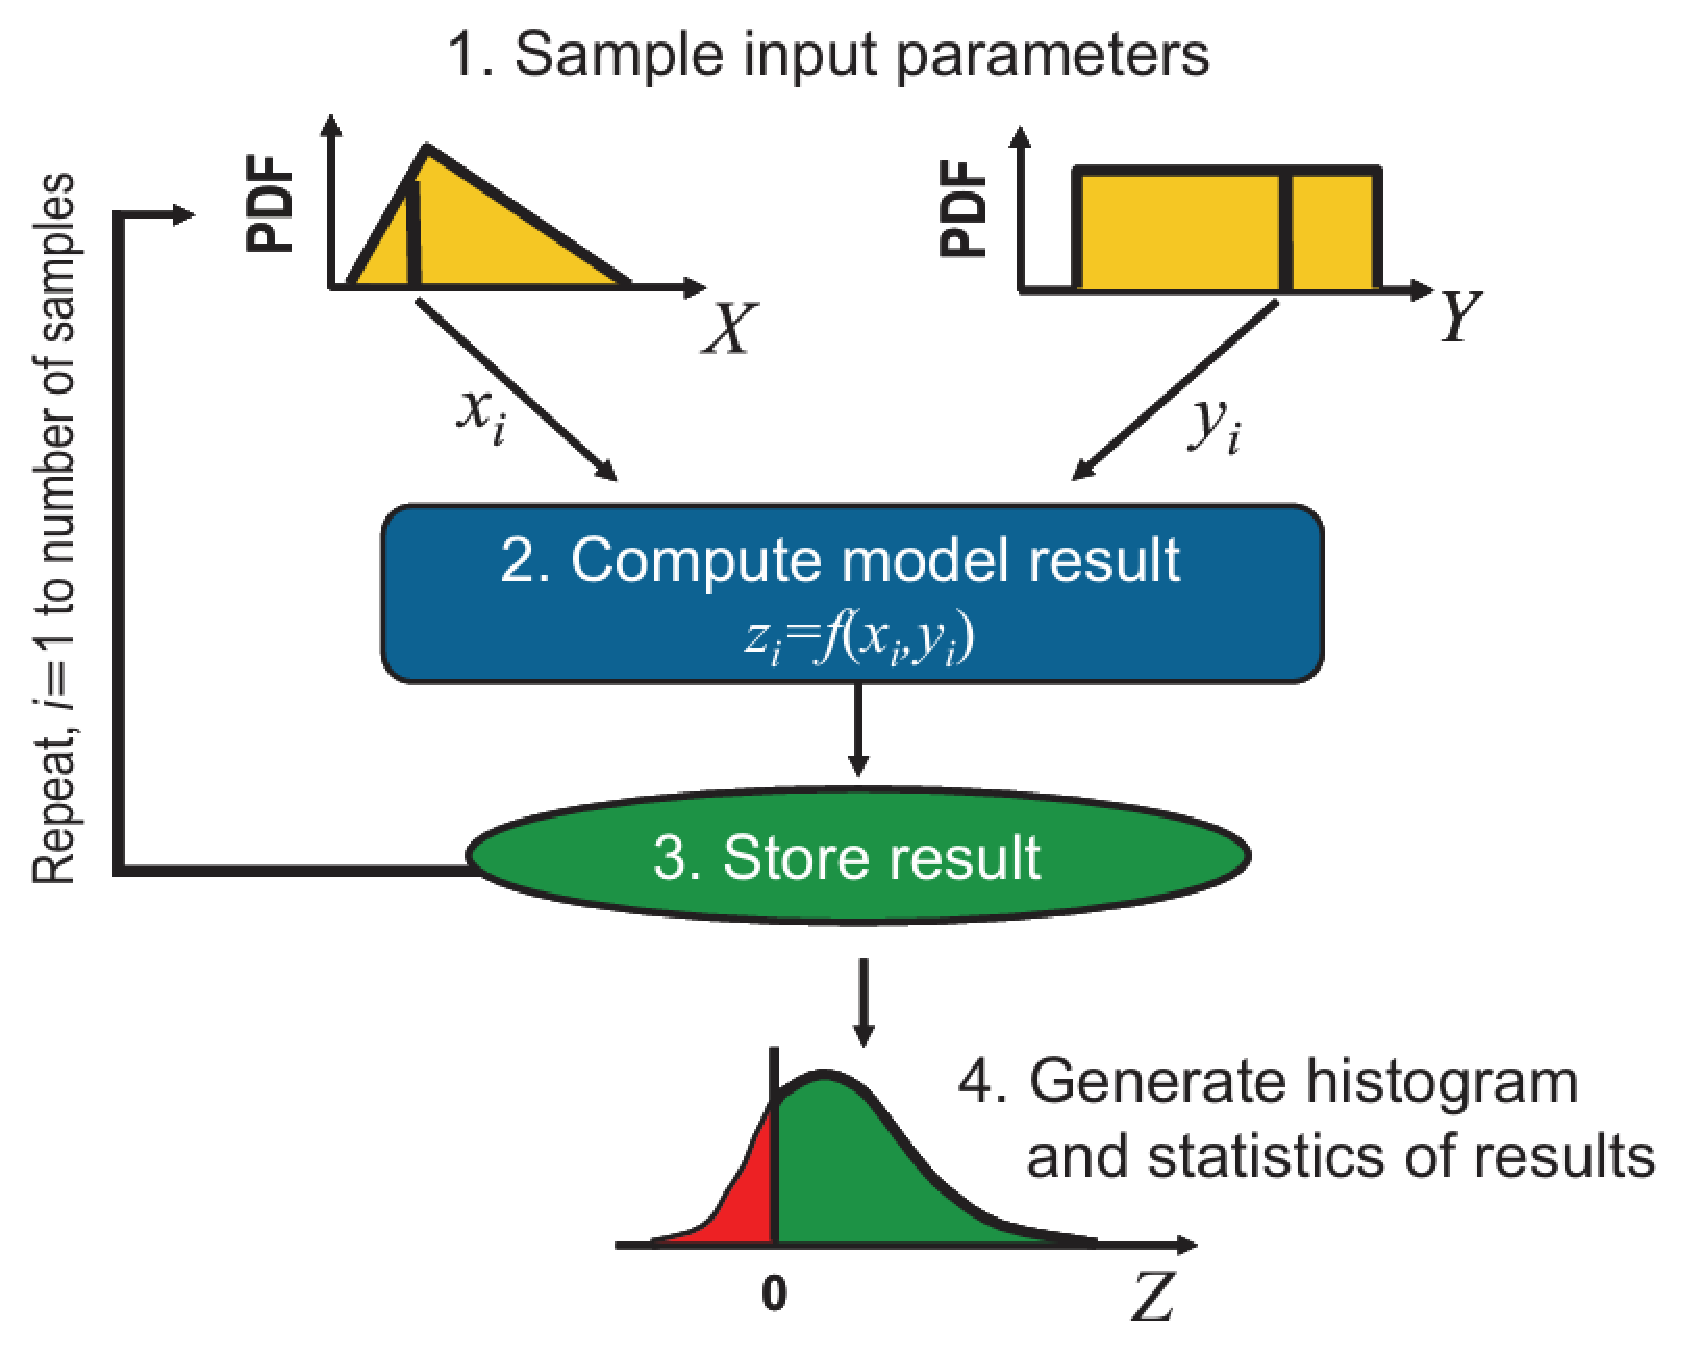
\includegraphics[width=\textwidth]{schematic_MCS.eps}
  \caption{Schematic of the Monte Carlo Simulation procedure. Source: Adapted from \cite{ref24}.}
  \label{fig6}
\end{minipage}
\end{figure}

One practical application of this method is the estimation of technical reserves by considering the uncertainties in parameters such as original oil in place (OOIP), technical recovery factor (TRF), and formation volume factor. The input distributions are generally informed by expert elicitation, and the resulting uncertainty in technical reserves can be effectively visualized using probabilistic output distributions—specifically, the probability density function (PDF) and cumulative distribution function (CDF), as depicted in Figure \ref{fig7}. A key theoretical point is that, especially in nonlinear models, the expected output value cannot be obtained simply by applying the model to the expected input values; instead, a full probabilistic analysis is necessary for reliable results.

\begin{figure}[H]
\centering
\begin{minipage}{0.85\textwidth}
  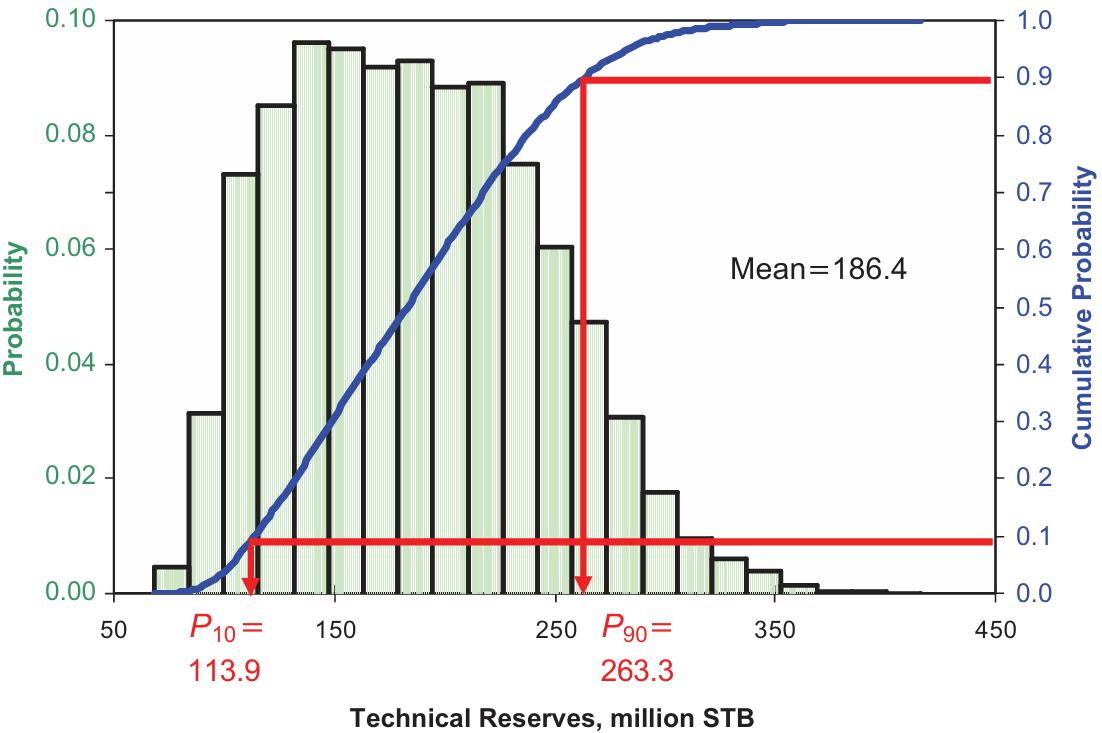
\includegraphics[width=\textwidth]{pdf_cdf.eps}
  \caption{PDF and CDF of technical reserves. Source: Adapted from \cite{ref24}.}
  \label{fig7}
\end{minipage}
\end{figure}

In this work, we will apply the MCS technique to quantify the uncertainty in the production curves generated by multiple realizations of the Egg model. This approach will enable a more rigorous assessment of the uncertainty associated with production forecasts, following the principles outlined by \cite{ref24}. 

\subsection{Geometric Brownian Motion}\label{subsec43}

In the present subsection, we give a brief description of the GBM process that is extensively used in the literature for modeling prices, especially in financial applications, commodity markets and option pricing \citep{ref25}. In the current paper, we employ the GBM to model variable operating costs. Originally developed by Black and Scholes for financial mathematics, the GBM provides a practical and tractable approach to represent the stochastic evolution of costs, mainly due to its simplicity and the small number of parameters required for calibration. 

\begin{definition}
A stochastic process $B(t)$ is a Brownian Motion if it satisfies the following:
\begin{enumerate}[label=(\roman*)]
    \item For any $t > s$, $v > u$ and $u > t$, the increments $B(t) - B(s)$ and $B(v) - B(u)$ are independent.
    \item Each increment is a zero-mean Gaussian random variable such that for all $t > s$, $B(t) - B(s) \sim \mathcal{N}(0, t-s)$.
    \item $B(0) = 0$.
\end{enumerate}
\end{definition}

The following theorem present the asset price dynamics that follows GBM.

\begin{theorem}
\theoremstyle{thmstyletwo}
A stochastic process $C(t)$ is said to follow a Geometric Brownian Motion (GBM) if its dynamics are governed by the following equation: 
\begin{equation}
dC(t) = \alpha C(t)\,dt + \sigma C(t)\,dB(t),
\label{eq1}
\end{equation}
\end{theorem} 
\noindent
where $B(t)$ is a Brownian Motion, $\alpha$ is the constant drift, and $\sigma$ is the constant volatility. $C(t)$ represents the current variable operating costs, $dC(t)$ change in price, $dt$ change in time, and $dB(t)=\epsilon \sqrt{dt}$, $\epsilon$ a Wiener process, which is normally distributed with a mean of zero and a standard deviation of $1$, $\mathcal{N}(0, 1)$. The solution for the stochastic differential equation \ref{eq1} for any arbitrary initial value $C(0)$ is given by:
\begin{equation}
C(t) = C(0) \exp\left[ \alpha t - \frac{1}{2} \sigma^2 t + \sigma B(t) \right].
\label{eq2}
\end{equation}

A positive drift ($\alpha > 0$) implies an upward trend in variable operating costs, whereas a negative drift ($\alpha < 0$) indicates a downward trend. The volatility parameter, $\sigma$, captures the uncertainty in cost evolution, with higher values leading to greater dispersion in possible future cost paths as time progresses. Figure \ref{fig10} illustrates examples of the simulated price paths and confidence bands based on 10,000 sumulated cases. We employ a GBM with a mean annual rate of increase of $\alpha=0.02$, a volatility of $\sigma=0.1$, and an initial variable operating cost of $\$10$ per barrel, as suggested by \cite{ref12}.

\begin{figure}[H]
\centering
\begin{minipage}{0.95\textwidth}
  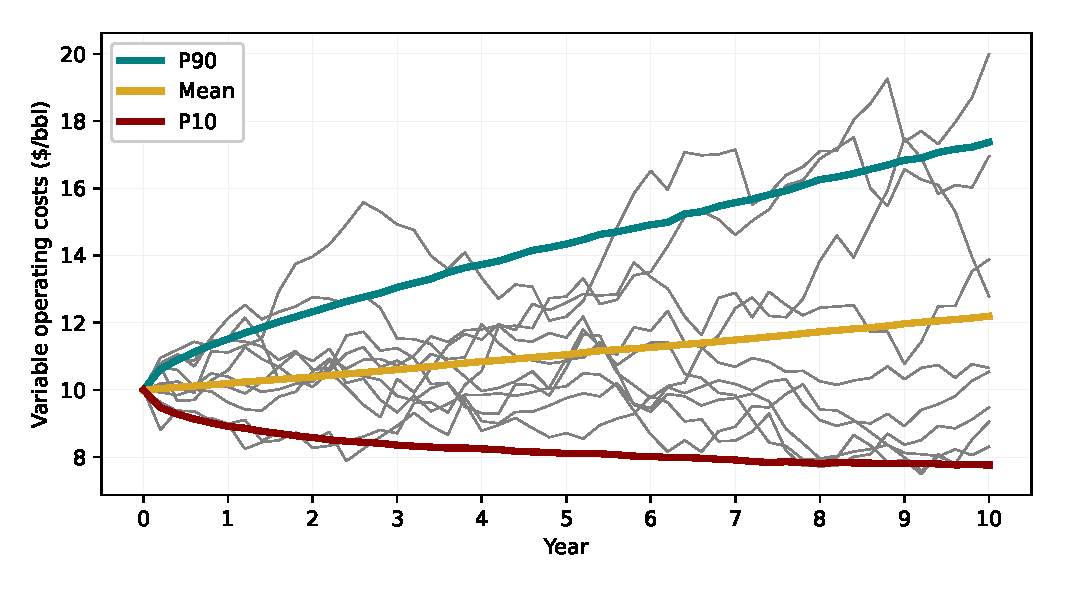
\includegraphics[width=\textwidth]{VOC_profile.eps}
  \caption{Variable operating costs simulations results, confidence bands and example price paths.}
  \label{fig10}
\end{minipage}
\end{figure}

%%\subsubsection{This is an example for third level head---subsubsection head}\label{subsubsec2}
\subsection{Two-Factor Model for Oil Prices}\label{subsec44}

Uncertainty in oil prices is a fundamental source of risk in the economic evaluation of E\&P projects. Traditional deterministic models, single-factor stochastic models, and even the widely-used GBM are often unable to capture the full richness and complexity of real oil price behavior, which is characterized by both short-term fluctuations and longer-term structural trends. To better represent these dynamics, we employ the two-factor model introduced by \cite{ref17}, which decomposes the logarithm of the oil price into short-term and long-term components.

In the Schwartz and Smith model, the long-term equilibrium component, denoted by $\xi_t$, is modeled as a GBM. This factor represents the persistent trend to which oil prices revert, capturing structural drivers such as technological innovation, depletion of reserves, inflation, and evolving market expectations. The short-term component, denoted by $\chi_t$, is modeled as a mean-reverting Ornstein-Uhlenbeck process, which reflects temporary deviations from equilibrium due to market shocks, geopolitical events, and supply-demand imbalances.

The risk-neutral dynamics of the two-factor model are described by the following system of stochastic differential equations:
\begin{equation}
    d\chi_t = (-\kappa \chi_t - \lambda_\chi)\,dt + \sigma_\chi\, d z_\chi, 
\label{eq:short_term}
\end{equation}
\begin{equation}
    d\xi_t = (\mu_\xi - \lambda_\xi)\,dt + \sigma_\xi\, d z_\xi, 
\label{eq:long_term}
\end{equation}
where
\begin{itemize}
    \item $\chi_t$ is the short-term deviation from equilibrium,
    \item $\xi_t$ is the long-term equilibrium component,
    \item $\mu_\xi$ is the drift of the long-term factor,
    \item $\kappa$ is the mean-reversion speed of the short-term factor,
    \item $\lambda_\chi$ and $\lambda_\xi$ are the risk premia for the short-term and long-term factors, respectively,
    \item $\sigma_\chi$ and $\sigma_\xi$ are the volatilities of the short-term and long-term factors, respectively,
    \item $d z_\chi$ and $d z_\xi$ are correlated increments of standard Brownian Motion processes with $d z_\chi d z_\xi = \rho_{\chi \xi} dt$.
\end{itemize}

The logarithmic oil price at time $t$ is then given by:
\begin{equation}
    \ln (P_t) = \chi_t + \xi_t,
    \label{eq:log_price}
\end{equation}
and the spot price itself can be recovered as:
\begin{equation}
    P_t = \exp(\chi_t + \xi_t).
    \label{eq:spot_price}
\end{equation}

For numerical implementation, the continuous-time stochastic differential equations \eqref{eq:short_term} and \eqref{eq:long_term} are discretized as follows \citep{ref16, ref21}:
\begin{equation}
    \xi_{t+1} = \xi_t + (\mu_\xi - \lambda_\xi)\Delta t + \sigma_\xi \varepsilon_\xi \sqrt{\Delta t},
    \label{eq:long_term_discrete}
\end{equation}
\begin{equation}
    \chi_{t+1} = \chi_t e^{-\kappa \Delta t} + \left(1 - e^{-\kappa \Delta t}\right) \frac{\lambda_\chi}{\kappa} + \sigma_\chi \sqrt{\frac{1-e^{-2\kappa\Delta t}}{2\kappa}} \varepsilon_\chi,
    \label{eq:short_term_discrete}
\end{equation}
where $\varepsilon_\xi$ and $\varepsilon_\chi$ are standard normal random variables, and $\Delta t$ is the time increment.

This modeling approach allows us to jointly capture both the short-term volatility and long-term trends observed in oil price dynamics. By adopting the two-factor model, the analysis can more accurately reflect the stochastic behavior of oil prices seen in historical data, thereby enabling more robust valuation, forecasting, and risk assessment for oil and gas investments.

The oil price model is characterized by seven parameters ($\kappa$, $\sigma_{\xi}$, $\sigma_{\chi}$, $\mu_{\xi}$, $\lambda_{\chi}$, $\lambda_{\xi}$, and $\rho_{\xi\chi}$), as well as two initial states, $\xi_0$ and $\chi_0$, which need to be estimated. Since these parameters are not directly observable in commodity markets, an appropriate calibration methodology is required. In this work, we follow the procedure proposed by \cite{ref26}, which utilizes the Kalman filter in conjunction with maximum likelihood estimation. The Kalman filter provides recursive estimates of the unobserved parameters by generating a posterior conditional distribution, given a time series of spot and futures prices and the corresponding measurement covariance matrix.

For our calibration, we use the yearly average of Brent crude oil futures prices from January 3, 2000, to March 7, 2025. Specifically, for each year, we observe six futures prices for contracts maturing in 1, 3, 5, 7, 9, and 13 months. Figure \ref{fig11} displays both observed and simulated expected futures prices using the calibrated parameters. The parameters resulting from the calibration are listed in Table \ref{tab4}.

 \begin{figure}[H]
\centering
\begin{minipage}{0.95\textwidth}
  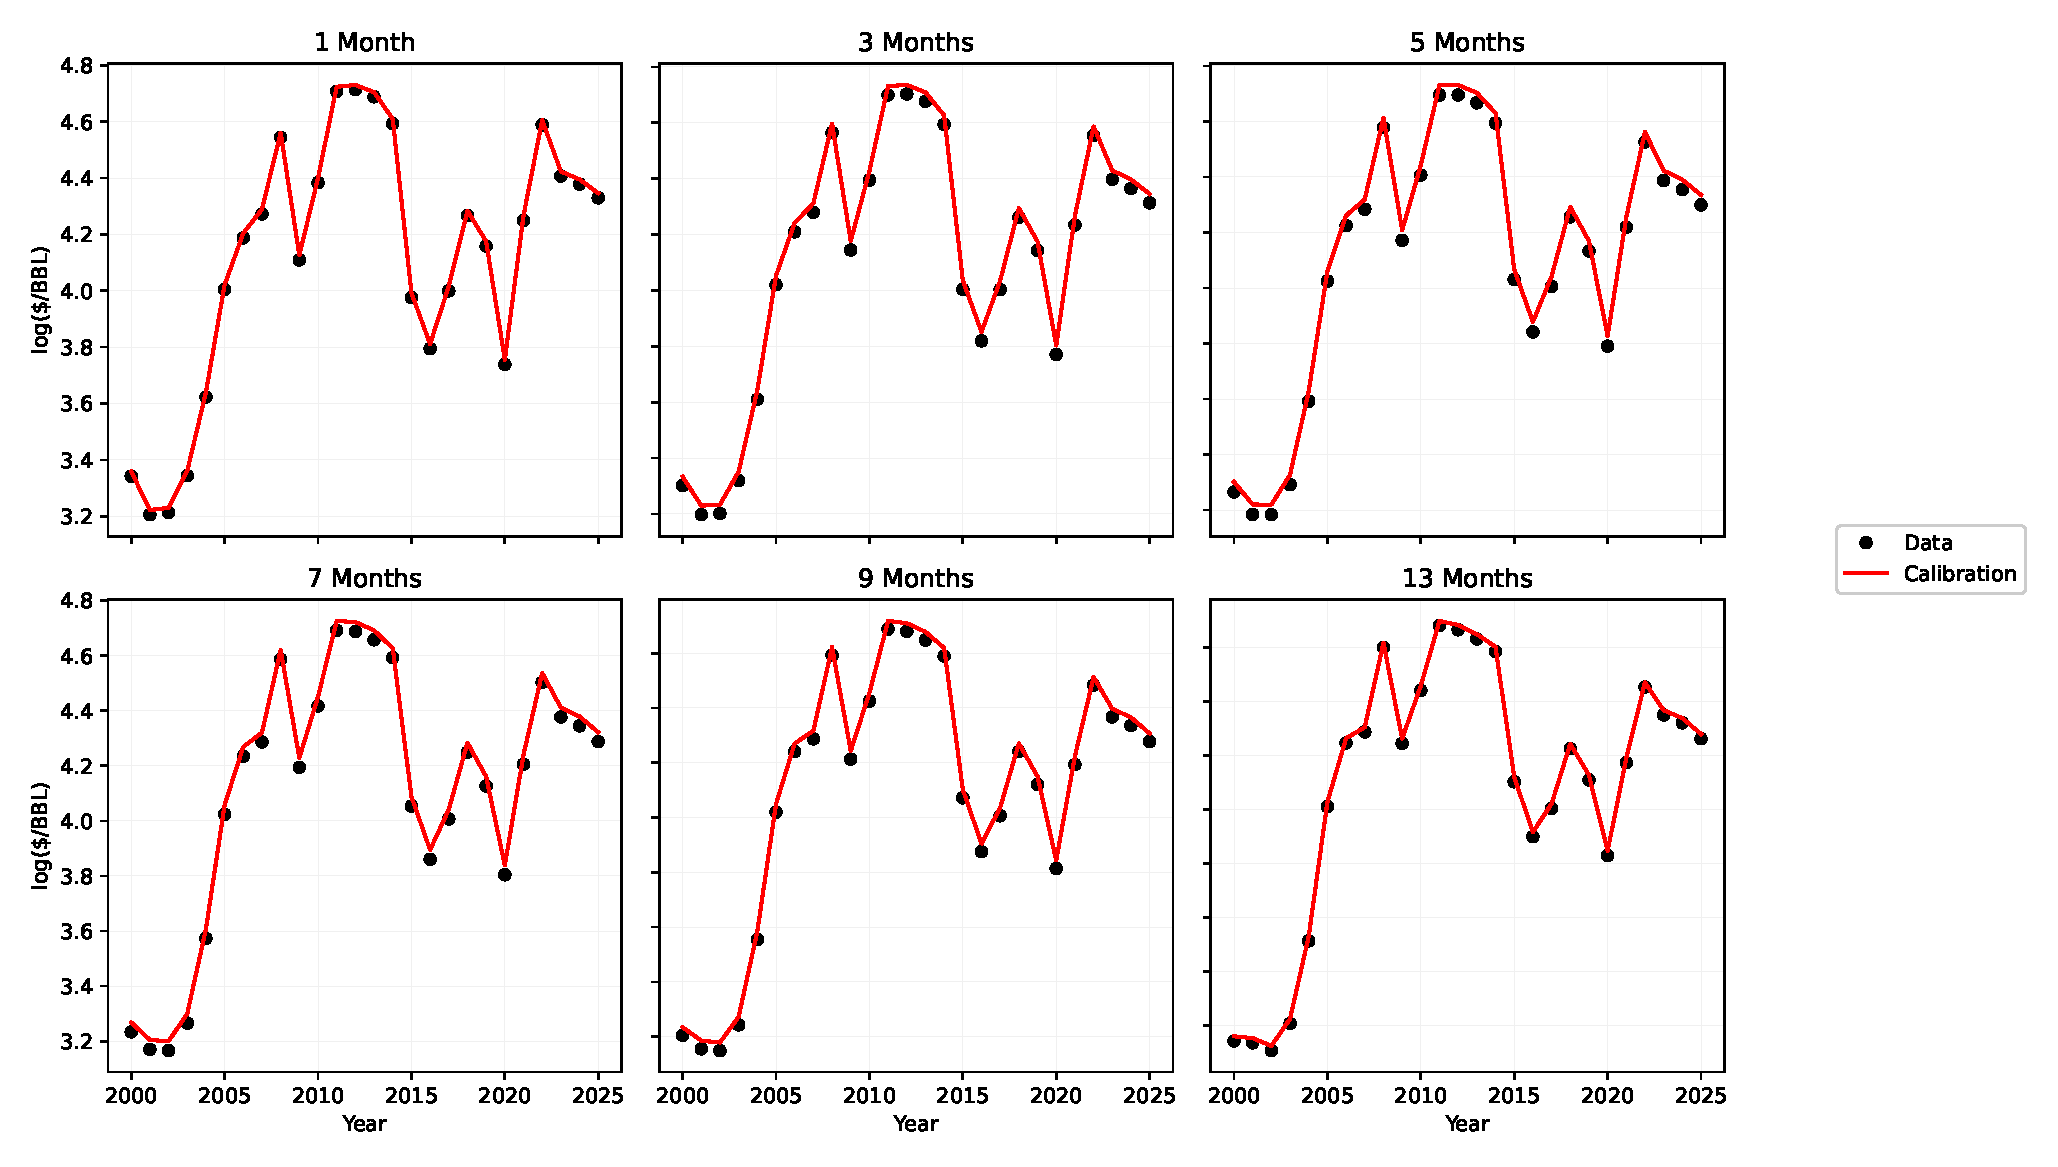
\includegraphics[width=\textwidth]{Price_Calibration.eps}
  \caption{Schwartz-Smith model calibration for oil prices.}
  \label{fig11}
\end{minipage}
\end{figure}

\begin{table}[h]
\centering
\caption{Schwartz-Smith model parameters from calibration}\label{tab4}%
\begin{tabularx}{10cm}{l *{11}{>{\centering\arraybackslash}X}}
\hline
\textbf{Parameter} & \textbf{Value} \\
\hline
$\kappa$       & 3.771 \\
$\sigma_\chi$  & 0.287 \\
$\chi_0$       & 0.049 \\
$\lambda_\chi$ & -0.202 \\
$\mu_\xi$      & -0.161 \\
$\sigma_\xi$   & 0.222 \\
$\xi_0$        & 4.207 \\
$\lambda_\xi$  & -0.092 \\
$\rho_{\chi\xi}$ & 0.398 \\
\hline
\end{tabularx}
\end{table}

\subsection{Least Squares Monte Carlo}\label{subsec45}

The valuation of real and financial options with early exercise features, such as American options, presents significant challenges due to the complexity of calculating the optimal value associated with the flexibility of exercise over time. LSM method, proposed by \cite{ref14}, is currently considered one of the most efficient algorithms for this type of problem, especially in situations with multiple sources of uncertainty and/or path dependence of the underlying asset \citep{ref16, ref15}. LSM method aims to approximate, on a path-by-path basis, the optimal stopping rule that yields the maximum possible value for an American option. For illustrative purposes, we consider the case in which early exercise is allowed only at a finite set of $K$ discrete times, $0 < t_1 \leq t_2 \leq \cdots \leq t_K = T$, and we determine the optimal exercise decision at each of these dates. While American options are often exercisable at any time prior to maturity, this continuous feature can be effectively handled in the LSM approach by choosing a sufficiently fine discretization (i.e., a large $K$), thereby closely approximating the continuous-time setting.

LSM approach involves comparing the immediate payoff of exercising the option before its expiration with the estimated value of continuing to hold the option. The decision to exercise is made whenever the immediate payoff exceeds the continuation value. The core idea of their method lies in estimating the conditional expectation of future payoffs using least squares regression, leveraging cross-sectional data obtained from MCS. At each potential exercise date, a regression is performed by relating the simulated continuation values to functions of the relevant state variables, thus approximating the conditional expectation at that moment. This cross-sectional dataset is constructed by simulating paths of the uncertain variables over time. The resulting estimation process allows for the approximation of the optimal exercise strategy along each simulation path, forming the foundation of what is now widely known as the LSM method \citep{ref14}.

LSM algorithm can be summarized in the following main steps \citep{ref14, ref15}:

\begin{enumerate}[label=(\roman*)]
\item A sufficiently large number of paths of the uncertain variables is generated by MCS.
\item At each exercise date, for the paths where the option is \textit{in the money}, a regression is performed of the future continuation values (obtained from the simulations) on functions of the state variables.
\item The basis functions for the Hilbert space of possible continuation values are typically chosen as orthogonal polynomials in $L^2$.
\item The fitted value from the regression is taken as an estimate of the conditional expected continuation value; this is then compared with the immediate payoff to determine whether the option should be exercised.
\item This procedure is applied recursively for all exercise dates, from maturity backward to the initial time.
\end{enumerate}

The space of square-integrable functions $L^2$ used in the LSM regression is a Hilbert space, for which there exists an orthonormal basis. In this paper, we use Laguerre polynomials as basis functions, which are defined as follows:
\begin{align}
L_0(x) &= \exp\left(-\frac{x}{2}\right), \\
L_1(x) &= \exp\left(-\frac{x}{2}\right) (1 - x), \\
L_2(x) &= \exp\left(-\frac{x}{2}\right) \left(1 - 2x + \frac{x^2}{2}\right), \\
L_n(x) &= \exp\left(-\frac{x}{2}\right) \frac{e^{x}}{n!} \frac{d^n}{dx^n} \left( x^n e^{-x} \right).
\end{align}

With these polynomials as basis functions, the continuation value function $F(\omega; t_{k-1})$ can be approximated by a linear combination of them:
\begin{equation}
F(\omega, t_{K-1}) = \sum_{j=0}^{\infty} a_j\, L_j(x),
\end{equation}
where the $a_j$ coefficients are constants. Other orthogonal polynomials, such as Hermite, Legendre, Jacobi, or Chebyshev polynomials, may also be used as basis functions \citep{ref14}. LSM approach presents fundamental advantages over other methods, as it is not very sensitive to the dimensionality of the problem (number of sources of uncertainty), and it is widely used in ROA in the oil and gas industry, since it can efficiently approximate dynamic programming for the selection of single or multiple exercise options \citep{ref15}.






\section{Results}\label{sec5}

\subsection{BDH problem}\label{subsec51}

The production profile reported in Table \ref{tab1} is also shown in Figure \ref{fig15}.

\begin{figure}[H]
\centering
\begin{minipage}{0.95\textwidth}
  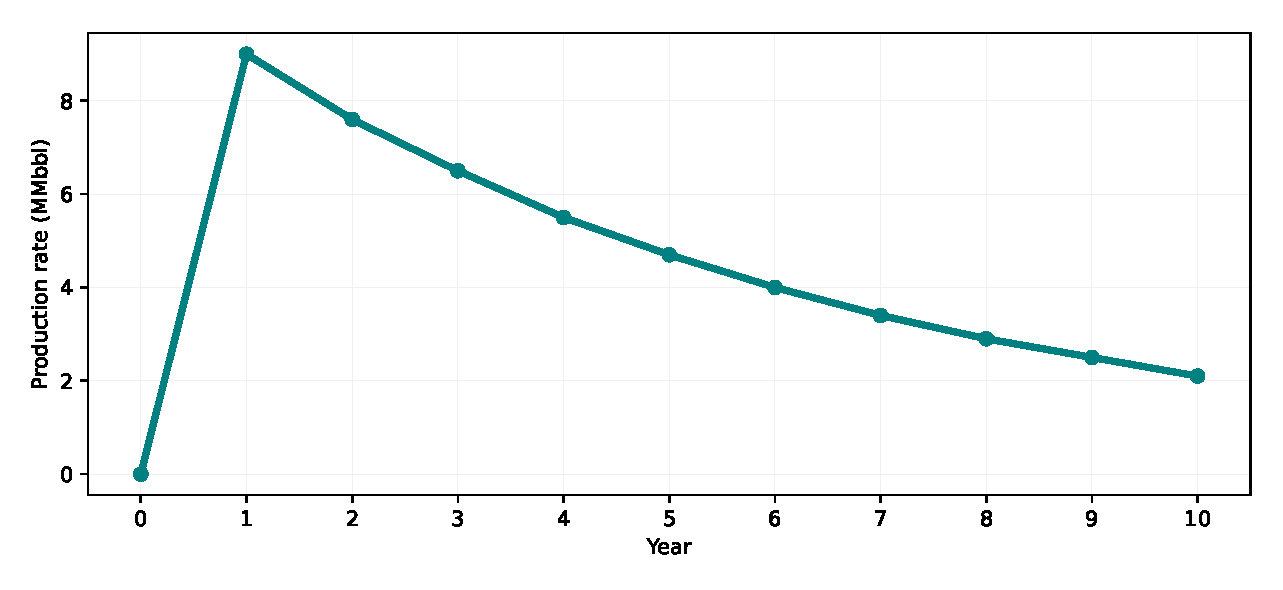
\includegraphics[width=\textwidth]{prod_profile.eps}
  \caption{Production profile for BDH problem.}
  \label{fig15}
\end{minipage}
\end{figure}

\subsection{Modified BDH problem}\label{subsec52}

\section{Conclusion}\label{sec6}



\bmhead{Acknowledgements}

Acknowledgements are not compulsory. Where included they should be brief. Grant or contribution numbers may be acknowledged.

Please refer to Journal-level guidance for any specific requirements.





%%===========================================================================================%%
%% If you are submitting to one of the Nature Portfolio journals, using the eJP submission   %%
%% system, please include the references within the manuscript file itself. You may do this  %%
%% by copying the reference list from your .bbl file, paste it into the main manuscript .tex %%
%% file, and delete the associated \verb+\bibliography+ commands.                            %%
%%===========================================================================================%%

\bibliography{sn-bibliography}% common bib file
%% if required, the content of .bbl file can be included here once bbl is generated
%%\input sn-article.bbl

\end{document}
